
\chapter{Stammdatenpflege}
\label{chap:data}

\section{Allgemeine Hinweise zur Datenpflege}

\subsection{Datensätze}

\subsubsection{Allgemeine Pflichtfelder}

Bei einzelne Datensätze ist \texttt{Name} ist ein einzigartiger Schlüsselwert, der das schnelle eintippen diese Ressource in Untis ermöglicht. Er soll dementsprechend so kurz und aussagekräftig wie möglich, gehalten werden. Der \texttt{Langname}, bzw. \texttt{Nachname}, hingegen enthält den tatsächlichen Namen der jeweilige Ressource. \textbf{Bei einzelne Datensätze sind die Name und Langname Angaben immer Pflicht}.\\

\subsubsection{Externer Name}
\label{sec:ext-name}

\texttt{Ext. Name} ist ein Fachbereich-übergreifender Schlüsselwert. Er ermöglicht die Sicht auf die Planung der Ressource außerhalb des eigenen Fachbereiches. Für Räume ist dieser Angabe ebenfalls Pflicht. Gruppen und Dozierende die für mehrere Fachbereiche interessant sind, wie der Studiengang Bioinformatik, die SuK Veranstaltungen für Fachbereich ME, grundsätzlich alle SuK Dozierende oder MNI Dozierende für Mathe, Physik, ... sollten ebenfalls eine solche externer Name haben. Sollte keinen externen Namen bereits für diese Ressourcen angelegt sein, schicke mir einen E-Mail und ich trage pflege den neuen externen Namen ein.


\subsection{Planungsabschnitte (Perioden)}

Planungsabschnitte werden mit der Ressource \texttt{Perioden} in Untis modelliert. Diese Ressourcen sind bereits eingepflegt. Man kann zwischen den jeweiligen Perioden mittels eine Auswahlbox in der obere Menüleiste zwischen den jeweiligen Perioden wechseln. Die Semester sind in der Regel der Hauptplanungsabschnitt an der THM, das Schuljahr hingegen ist für die Pflege von Stammdaten gedacht.\\

\newpage

\begin{wrapfigure}{r}{0.25\textwidth}
	\vspace{-4pt}
	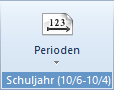
\includegraphics[width=.24\textwidth,right]{perioden}
	\vspace{-15pt}
	\caption{Perioden}
	\label{fig:mf-sg}
\end{wrapfigure}

\noindent
\textbf{Die Pflege von Gruppen, Räume und Dozenten muss in der Periode ``Schuljahr" gemacht werden.} Wenn Daten in der Schuljahr Periode eingepflegt sind, werden die neuen Daten, bzw. Änderungen, automatisch im Winter- und Sommersemester Perioden ersichtlich. Sollten neue Stammdaten oder Änderungen auf bestehenden in die Winter- oder Sommersemester Perioden eingepflegt werden, sind diese Daten nur in diese eine Periode ersichtlich. Das führt zwangsläufig zu Dateninkonsistenzen.\\

\section{Spezielle Ressourcen}

Spezielle Ressourcen sind welche, die als Attribute in andere verwendet werden, Studiengänge und Beschreibungen. Die Stammdatenpflege dieser Ressourcen erreicht man am leichtesten in dem man \texttt{Dateneingabe} in Reiterleiste auswählt, \texttt{Sonstige Daten} aufklappt und \texttt{Studiengänge} oder \texttt{Beschreibungen} auswählt.\\

\begin{figure}[h]
	\centering
	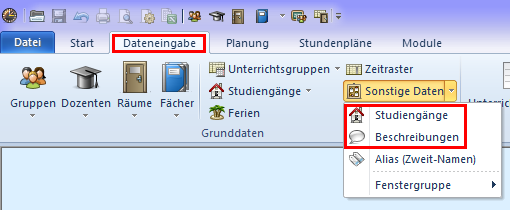
\includegraphics[width=.8\textwidth]{spezielle-daten-menu}
	\vspace{-5pt}
	\caption{Menüführung: spezielle Daten}
	\label{fig:spezielle-daten-menu}
\end{figure}

\subsection{Studiengänge (Abteilungen)}

Studiengänge werden an der THM Gruppen zugeordnet. Die damit implizierte Aussage ist Gruppen gehören Studiengänge. Man könnte auch Dozenten, Räume und Fächer Studiengänge zuordnen. Dies würde wegen unsere weitere Modellierung keine weitere Auswirkung haben.\\
\\
Sollte man die THM Organizer Komponente verwenden um die Stundenpläne auf der Webseite darzustellen werden diese Angaben verwendet für die Knoten des Navigationsbaums für die Gruppenpläne.\\

\newpage

\begin{wrapfigure}{r}{0.4\textwidth}
	\centering
	\vspace{-4pt}
	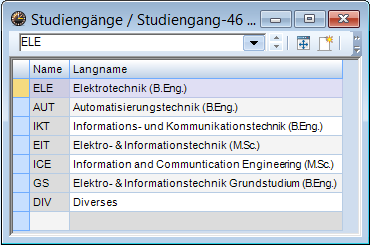
\includegraphics[width=.38\textwidth]{studiengange}
	\vspace{-5pt}
	\caption{Studiengänge}
	\label{fig:studiengange}
\end{wrapfigure}

\noindent
\texttt{Name}: Die typische Schreibweise besteht aus ein paar Buchstaben, die der Name andeuten. Im Falle Zweideutigkeit, z.B. der gleiche Name für einen Bachelor und einen Master Studiengang, wird typischerweise die erste Buchstabe der Abschluss nach einem Punkt angehängt.\\

\noindent
\texttt{Langname}: Der Name des Studiengangs mit offizieller Abkürzung des Abschlusses in runden Klammern dahinter. Dieser Wert wird öffentlich verwendet in die Darstellungen von Untis und THM Organizer.\\

\subsection{Beschreibungen}

An der THM wird diese Ressource um Fachkompetenzen, Raumkategorien und Unterrichtsmethoden zu modellieren. In Untis gibt es teilweise ähnliche Angaben, sie lassen sich aber nicht einstellen und sind deshalb nicht zu gebrauchen.\\

\noindent
{\large Attributes\par}
\vspace{8pt}

\begin{wrapfigure}{r}{0.4\textwidth}
	\centering
	\vspace{-19pt}
	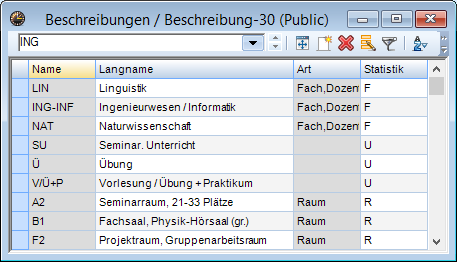
\includegraphics[width=.38\textwidth,right]{beschreibungen}
	\vspace{-15pt}
	\caption{Beschreibungen}
	\label{fig:beschreibungen}
	\vspace{-5pt}
\end{wrapfigure}

\noindent
\texttt{Art}: Dieser Angabe ist nicht zu gebrauchen und kann nicht ausgeblendet werden. Bitte ignorieren.\\
\\
\texttt{Statistik}: Der Statistik Angabe wird von uns um die tatsächliche Verwendung festzulegen verwendet. (Pflicht)\\

\subsection{Fachkompetenzen}
\label{subsec:fachkompetenzen}

Kompetenzen sagen was aus über den groben Inhalt von Gruppen und Fächer, oder die Themengebiete in der sich ein Dozent ein Experte ist.\\
\\
Derzeit sind die Namen und Langnamen nach einem von Herr Kneisel entworfenes System aufgebaut. Demnach besteht ein Fachkompetenz aus Basis-Kompetenzen, die jeweils durch drei Buchstaben gekennzeichnet sind. Diese entsprechen ein recht grobes Themengebiet wie Naturwissenschaft oder Bauingenieurwesen. Zusätzlich gibt es die Möglichkeit Hybride-Kompetenzen zu erschaffen. Die Namen dieser werden durch die Bezeichner von zwei Basis-Kompetenzen verbunden durch einem Minus-Zeichen gebildet. Ihre Langnamen entsprechend durch die der zwei Basis-Kompetenzen durch `` / " getrennt. In der Statistik Spalte soll die Buchstabe ``F" eingepflegt werden.\\

\newpage

\begin{quote}
	\textit{Hier wäre eine Überarbeitung des Systems grundsätzlich erwünschenswert. Beispielsweise hat Fachbereich Wirtschaft, zusätzlich zu den Einträgen vom Kneisel'sche System, neun Schwerpunkte, wie Mittelstand oder Marketing. Diese sind um einiges aussagekräftiger und relevanter sowohl für Studenten als auch für Dozenten.}
\end{quote}

\noindent
THM Organizer verwendet diese Angaben für die Stundenplan Navigation für Dozenten und Fächer.\\

\subsection{Raumkategorien}
\label{subsec:room-category}

Der Name und der Langname beziehen sich auf einem System entwickelt von Herr Deniffel für die THM, wonach die Namen etwas über der Raumtyp aussagen und Andeutungen auf dessen Kapazität oder Ausstattung machen.\\
\\
Der Name besteht meist aus einer Buchstabe und einer Zahl. Zum Beispiel ``A" deutet auf ein Seminarraum oder Hörsaal, wohingegen ``D" ein Rechnerraum kennzeichnet. Die Zahlen beziehen sich auf Raumeigenschaften wie Größe oder Ausstattung. Bei A2 heißt das ``2" 21 bis 33 Sitzplätze, bei D2 hingegen heißt die ``2", dass in dem Raum eine fachspezifische Ausstattung sich befindet. Der Langname ist eine von Kommata getrennte Auflösung dieser zwei Teile. Bei Raumkategorien wird ein ``R" in der Statistik Spalte eingetragen.\\
\\
Eine vollständige Liste der Raumkategorien befindet sich im \secref{sec:dennifel}.\\
\\
THM Organizer verwendet diese Angaben für die Stundenplan Navigation für Räume.\\

\subsection{Unterrichtsmethoden}

Unterrichtsmethoden beschreiben der Lehrform eines Unterrichts.\\

\begin{wrapfigure}{r}{0.35\textwidth}
	\vspace{-14pt}
	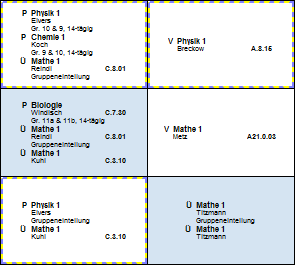
\includegraphics[width=.34\textwidth]{MethodsUntis}
	\vspace{-5pt}
	\caption{Mögliche Darstellung von Unterrichtsmethoden in Untis}
	\label{fig:methoden-untis}
	\vspace{-5pt}
\end{wrapfigure}

\noindent
Der Name besteht meist aus einer Buchstabe, wie ``V" für Vorlesung oder ``L" für Labor. Der Langname entsprechend der ausführliche Schreibweise. Sollte ein Unterricht mehrere Methoden verwenden, können auch hier Hybride-Methoden erschaffen werden, in dem man die einfachen Angaben durch ein ``/" trennt. Beispielsweise ``V/Ü"  für Vorlesung oder Übung, oder ``S/P" für Seminar oder Praktikum. Für Unterrichtsmethoden ist die entsprechende Statistik Angabe ``U".\\
\\
In Untis können diese Angaben so eingerichtet werden, dass sie auch mitausgegeben werden. Eine mögliche Darstellung finden Sie in \figref{fig:methoden-untis}. In THM Organizer wird diese Angabe als Teil des Unterrichtsnamen immer ausgegeben.\\

\section{Gruppen}

\begin{wrapfigure}{r}{0.08\textwidth}
	\vspace{-70pt}
	
\includegraphics[width=.08\textwidth]{gruppen-menu}
\end{wrapfigure}

\vspace{25pt}

Gruppen, auch Klassen in Untis genannt, sind zugleich Zielgruppe und Angebot für eine Menge an Unterrichten, und werden nach das eine oder das andere genannt. Zum Beispiel eine Gruppe mit der Name ``1. Semester" oder ``Schwerpunkt Wirtschaftsinformatik" bezeichnet sowohl die Gruppe von Studenten die eine Gruppe von Unterrichte besuchen soll, als auch die Menge an Unterrichte die diese Studenten besuchen.\\
\\
Die Stammdatenpflege der Gruppen erreicht man in dem man in der Reiterleiste \texttt{Start} aktiviert hat, \texttt{Gruppen} aufklappt und \texttt{Stammdaten} auswählt. Stellen Sie auch vorerst sicher, dass die \texttt{Periode} ``Schuljahr" ausgewählt ist.

\begin{figure}[h]
	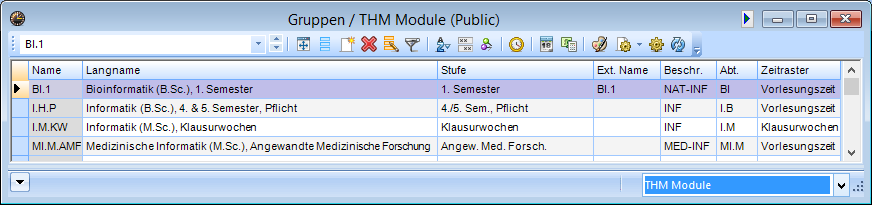
\includegraphics[width=1\textwidth]{Gruppen}
	\vspace{-15pt}
	\caption{Gruppen}
	\label{fig:groups}
\end{figure}

\noindent
{\large Attributes\par}
\vspace{8pt}

\noindent
\texttt{Name}: Beinhaltet Hinweise auf den jeweiligen Studiengang, sowie die spezifische Untergliederung dessen. Typischerweise mit Punkten getrennt.\\

\noindent
\texttt{Langame}: Der ausgeschriebene Name des Studiengangs mit Abschluss in runden Klammern, gefolgt von Untergliederungsteile, getrennt durch Kommas.\\

\noindent
\texttt{Ext. Name}: (Pflicht bei Fachbereichsübergreifende Gruppen, sonst Optional, sehe auch 
\secref{sec:ext-name})\\

\noindent
\texttt{Stufe}: Eine Kurzfassung der Untergliederung. Diese Angabe wird als Plan Name in der Navigation in THM Organizer benutzt.(Pflicht)\\

\noindent
\texttt{Beschr.} (Fachkompetenz): Assoziiert die Gruppe mit einem Fachkompetenz. (Pflicht, sehe \secref{subsec:fachkompetenzen}))\\

\noindent
\texttt{Abt.} (Studiengang): Assoziiert die Gruppe und ihre Unterrichte mit einem Studiengang. (Pflicht)\\

\noindent
\texttt{Zeitraster}: Assoziiert die Gruppe mit einem Zeitraster. Standardmäßig ist der Wert dieser Spalte ``Hauptzeitraster". Falls Multi-Zeitraster verwendet wird, kann man eingepflegte Zeitraster auswählen. (Pflicht, wird automatisch mit einem default Wert gefüllt, sehe auch \nameref{sec:zeitraster})

\subsubsection{Zeitraster \& Klausurwochen}
\label{sec:zeitraster}

Zeitraster legen die Blöcke fest in dem man Unterrichtsinstanzen unterbringen kann. An der THM haben wir bisher zwei feste Zeitraster, eine für Vorlesungen und eine für die Klausurwochen. Solche Zeitraster sind in Untis mit Gruppen assoziiert. Diese hat Konsequenzen für unsere Modellierung der Klausurwochen, denn wenn Zeitraster nur mit Gruppen assoziert werden können, muss es sinnvolle Gruppen geben um die Klausuren der Klausurwochen zu modellieren.\\
\\
In Fachbereich MNI haben wir, eine Klausurwochen-Gruppe pro Studiengang angelegt. Diese haben verwenden die zweistündige Zeitraster der Klausurwochen. Klausuren können damit Untis intern sehr gut geregelt werden. Es ist aber so, dass die zusätzliche Zeitraster werden noch nicht mit exportiert und kann in Organizer deshalb noch nicht angezeigt werden.\\

\section{Dozenten}

\begin{wrapfigure}{r}{0.08\textwidth}
	\vspace{-70pt}
	
\includegraphics[width=.08\textwidth]{dozenten-menu}
\end{wrapfigure}

\vspace{25pt}

Dozenten, auch Lehrer in Untis genannt, bezeichnen Festangestellte Dozenten, Lehrbeauftragte, Tutoren, Vortragende, Seminarleiter. Kurz gesagt, alle die für eine Veranstaltung oder Unterricht verantwortlich sind.\\
\\
Sie erreicht man von der \texttt{Start} Leiste in dem Man \texttt{Dozenten} aufklappt und \texttt{Stammdaten} auswählt.\\

\begin{figure}[h]
	\centering
	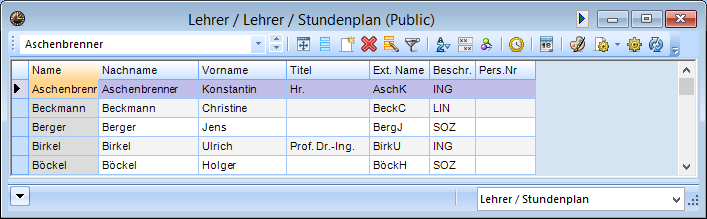
\includegraphics[width=.8\textwidth]{Teachers}
	\vspace{-5pt}
	\caption{Dozenten}
	\label{fig:teachers}
\end{figure}

\noindent
{\large Attributes\par}
\vspace{8pt}

\noindent
\texttt{Name}: Typischerweise gleich der Nachname, bei Uneindeutigkeiten werden Buchstaben aus den Vornamen und anderen Nachnamen hinzugefügt.\\

\noindent
\texttt{Nachname}: Die Nachnamen des Dozenten.\\

\noindent
\texttt{Vorname}: Die Vornamen des Dozenten.(Empfohlen)\\

\noindent
\texttt{Titel}: Der Title des Dozenten.(Optional)\\

\noindent
\texttt{Ext.Name}: (Pflicht bei Dozenten die in mehreren Fachbereiche tätig sind, sonst Optional, sehe auch 
\secref{sec:ext-name})\\

\noindent
\texttt{Beschr.} (Kompetenz): Assoziiert der Dozent mit einem Fachkompetenz. (Pflicht, sehe   \secref{subsec:fachkompetenzen}))\\

\noindent
\texttt{Pers.Nr} (THM Benutzerkennung): Die THM Benutzerkennung des Dozenten. Verhilft die eindeutige Zuordnung des Dozenten und ermöglicht ggf. die Verlinkung auf einem Benutzer-Profile aus THM Organizer. (Optional)\\

\section{Räume}

\begin{wrapfigure}{r}{0.08\textwidth}
	\vspace{-80pt}
	
\includegraphics[width=.08\textwidth]{raume-menu}
\end{wrapfigure}

\vspace{35pt}

Räume bezeichnen sämtliche Orte wo Unterrichte, Vorträge, Sitzungen und sonstige Stundenplan relevante Ereignisse stattfinden. Obwohl stereotypische Räume wie Hörsäle, Besprechungsräume, Labore machen den Großteil der Raumbestand aus, auch außergewöhnliche Ortschaften wie der Grillplatz, Kongresshalle, Krankenhäuser, oder gar ``Online" sind auch vertreten.\\
\\
Von der \texttt{Start} Leiste drückt man klappt man \texttt{Räume} auf und wählt \texttt{Stammdaten} aus.

\begin{figure}[h]
	\centering
	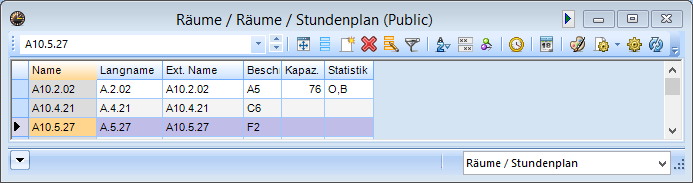
\includegraphics[width=.8\textwidth]{Rooms}
	\vspace{-5pt}
	\caption{Räume}
	\label{fig:rooms}
\end{figure}

\noindent
{\large Attributes\par}
\vspace{8pt}

\noindent
\texttt{Name}: Der Raum Name. Damit die Namen Campus-übergreifend eindeutig sind, wird der Bezeichner für A und C Gebäuden zu ``A10", bzw. ``C10".\\

\noindent
\texttt{Langname}: Die aktuelle Bezeichnung für den Raum.\\

\noindent
\texttt{Ext.Name}: Das Selbe wie der \texttt{Name}. (Pflicht)\\

\noindent
\texttt{Beschr.} (Raumkategorie): Die Kategorie des Raumes. Wird in THM Organizer für die Navigation unter den Raumpläne. (Pflicht, sehe \secref{subsec:room-category})\\

\noindent
\texttt{Kapaz.} (Kapazität): Die Anzahl der Sitzplätze / Rechnerplätze. (Optional)\\

\noindent
\texttt{Statistik} (Ausstattung): Einstellige Bezeichner für die Raumausstattung, wie Overhead (O) oder Beamer (B). Die Bezeichner werden durch Kommata getrennt. Diese werden von Untis eingefügt, der Benutzer braucht nur die Buchstaben einzutragen. (\textbf{Optional})\\

\subsubsection{Raumgruppen}

Raumgruppen sind Gruppierungen von Räumen nach Typ, Ausstattung, Kapazität, Verwendungszweck, eine Kombination daraus, oder was man sonst noch einfällt. In \figref{fig:roomgroups} sieht man drei der Gruppen die Fachbereich MNI verwendet. Die erst Gruppe, LPC, beinhaltet eine Auflistung der Rechnerlabore in Gebäude A20, jeweils von gleichen Typ, mit einer ähnlichen Ausstattung und Kapazität.\\
\\
Raumgruppen an sich sind optional. Sie sind lediglich eine Hilfestellung zur Raumsuche. Sie werden in der Lehrplanung eingetragen und, sofern die Räume der Raumgruppe nicht erschöpft sind, muss man erst gar nicht nach einem geeigneten Raum suchen. Mehr Dazu später in !!!!!!.\\
\\ 
Von der \texttt{Start} Leiste drückt man klappt man \texttt{Räume} auf und wählt \texttt{Raumgruppen} aus.

\begin{figure}[h]
	\centering
	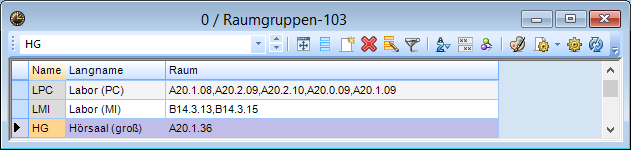
\includegraphics[width=.8\textwidth]{RoomGroups}
	\vspace{-5pt}
	\caption{Raumgruppen}
	\label{fig:roomgroups}
\end{figure}

\noindent
{\large Attributes\par}
\vspace{8pt}

\noindent
\texttt{Raum}: Eine Komma-getrennte Liste der Räume, die dieser Gruppe gehören. (Pflicht, sofern verwendet)\\

\section{Fächer}

\begin{wrapfigure}{r}{0.08\textwidth}
	\vspace{-80pt}
	
\includegraphics[width=.08\textwidth]{facher-menu}
\end{wrapfigure}

\vspace{35pt}

Fächer sind die Namensträger für Unterrichte und Unterrichtsinstanzen. Sie geben einen Hinweis darauf, welche Lerninhalte in einem Unterricht oder Unterrichtsinstanz übermittelt werden. Der Begriff Fächer bezeichnet hier auch Module sofern diese der gewünschte Name für die Ausgabe ist.\\
\\
Zum Beispiel besteht das Modul International Marketing im Studiengang Unternehmensführung aus mehrere Fächer, im Stundenplan ist nur einer Name für alle solche Fächer gewollt. Im Gegensatz dazu stehen Module wie Theorie des Entwerfens I aus Studiengang Bauingenieurwesen, hier sind die Namen der untergeordneten Fächer Einführung ins Entwerfen und Baugeschichte der Ausgabe gewollt und müssen deshalb getrennt eingepflegt werden.\\
\\ 
Fächer haben die besondere Eigenschaft, dass sie nicht im Schuljahr-Periode gepflegt werden müssen, denn jegliche Änderungen an einem Fach sind sofort in allen Perioden sichtbar.\\
\\
Um diese zu erstellen oder bearbeiten, muss man in der \texttt{Start} Leiste \texttt{Fächer} aufklappen und \texttt{Stammdaten} auswählen.

\begin{figure}[h]
	\centering
	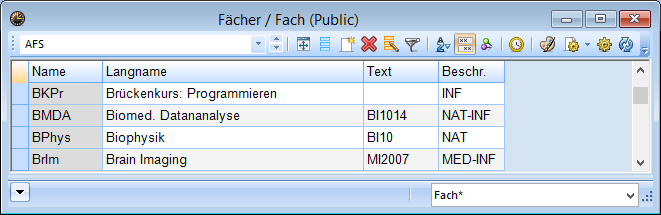
\includegraphics[width=.8\textwidth]{Subjects}
	\vspace{-5pt}
	\caption{Fächer}
	\label{fig:subjects}
\end{figure}

\noindent
{\large Attributes\par}
\vspace{8pt}

\noindent
\texttt{Text} (Modulnummer): Die Modulnummer des Faches/Moduls. Hier ist entscheidend, wie die Modulen in LSF abgelegt werden, denn diese Angabe verhilft die Weiterleitung auf Modulbeschreibungen. Sollten Module nicht atomar gehalten werden, weißt man nicht unbedingt ob die Beschreibungen auf der Ebene der Module oder auf Ebene des Faches liegen. Im Zweifelsfall pflegen wir diese Angaben gemeinsam.(Empfohlen)\\

\noindent
\texttt{Beschr.} (Kompetenz): Assoziiert das Fach mit einem Kompetenz. (Pflicht, sehe \secref{subsec:fachkompetenzen})\\

\newpage

\section{Unterrichtsgruppen}

\noindent
Unterrichtsgruppen sind Rahmen für die zeitliche Verlauf von Unterrichte. Dort kann man feste Start- und Enddaten angeben, sowie der Verlauf innerhalb diese zwei Daten.\\

\begin{wrapfigure}{r}{0.35\textwidth}
	\vspace{-14pt}
	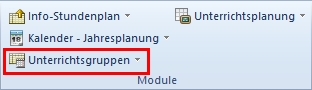
\includegraphics[width=.34\textwidth]{unterrichtsgruppen-symbol}
	\vspace{-5pt}
	\caption{Unterrichtsgruppen im Menü}
\end{wrapfigure}

\noindent
Unterrichtsgruppen findet man in der \texttt{Start} Leiste im Rubrik \texttt{Module}. Es sind bereits in jede Schule Unterrichtsgruppen eingetragen und konfiguriert, daher wird es eure Aufgabe diese die Gegebenheiten eure Fachbereiche anzupassen. Beispiele für Unterrichtsgruppen findet man in 
\secref{sec:unterrichtsgruppen-values}.\\


\begin{wrapfigure}{r}{0.35\textwidth}
	\vspace{-14pt}
	\label{fig:unterrichtsgruppen-symbol}
	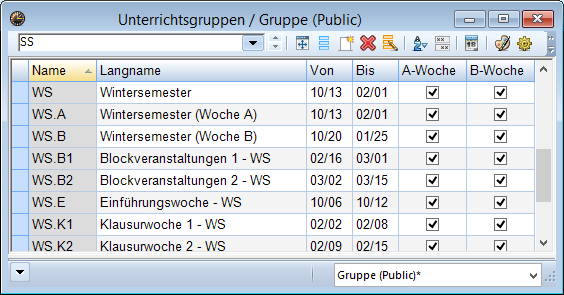
\includegraphics[width=.34\textwidth]{unterrichtsgruppen-ansicht}
	\vspace{-5pt}
	\caption{Unterrichtsgruppen Ansicht}
	\label{fig:unterrichtsgruppen-ansicht}
	\vspace{14pt}
	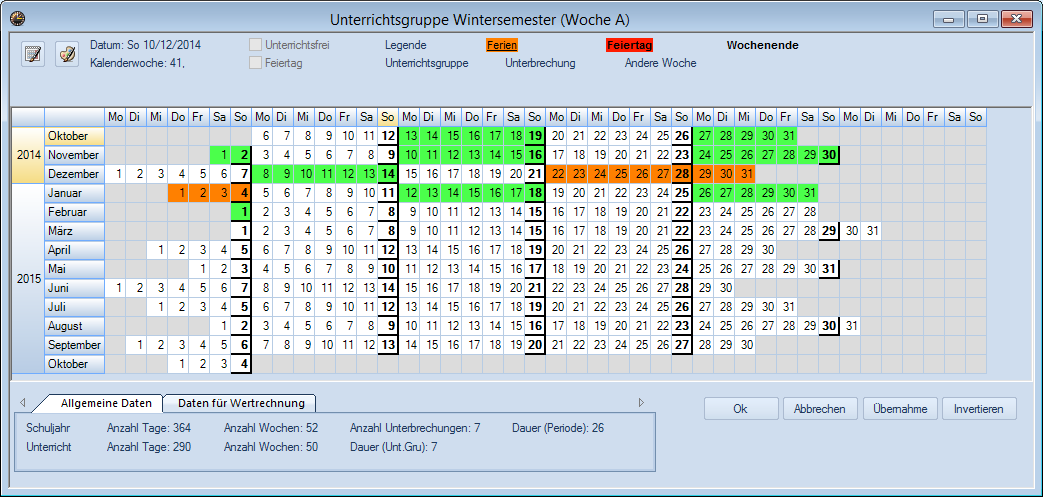
\includegraphics[width=.34\textwidth]{unterrichtsgruppen-kalender-ansicht}
	\vspace{-5pt}
	\caption{Unterrichtsgruppen Kalender}
	\label{fig:unterrichtsgruppen-kalender-ansicht}
\end{wrapfigure}

\noindent
{\large Attributes\par}
\vspace{8pt}

\noindent
\texttt{Von}: Das Startdatum der Unterrichtsgruppe. (Pflicht)\\

\noindent
\texttt{Bis}: Das Enddatum der Unterrichtsgruppe. (Pflicht)\\

\noindent
{\large Kalender\par}
\vspace{8pt}

\noindent
Was Unterrichtsgruppen von der Datenpflege besonders macht ist die Feinjustierung. Um akkurate Unterrichtsverläufe einzupflegen reichen diese Start- und Enddaten selten aus. Daher muss man hier meistens den Schuljahreskalender-Ansicht verwenden. Im Kalender Ansicht kann man Datenbereiche überstreichen oder einzelne Tage anklicken um diese in den Verlauf der Unterrichtgruppe zu übernehmen oder entfernen. Schliesslich klickt man auf \texttt{Ok} oder \texttt{Übernahme} um die Änderungen geltend zu machen.






